\input{dfki.defs}

\title[Simulation in Robotics]{Lecture 3 - Simulation of Techniques and Tools}
\author{Julius Martensen}
\date{\today}

\begin{document}


  \frame{\titlepage}

  \section[\Overview]{}
  % Talk about the targets
  % Refer to Christoph and Bernd
  % Give an outline to the lectures

  \frame{\tableofcontents}

  \section{Motivation}
  % Robots are mechatronic systems
  % They are highly interactive
  % The world around them is not

  \section{A holistic perspective}

  \frame{
    \frametitle{Robotics - An Interdisciplinary Science}

    \begin{figure}
      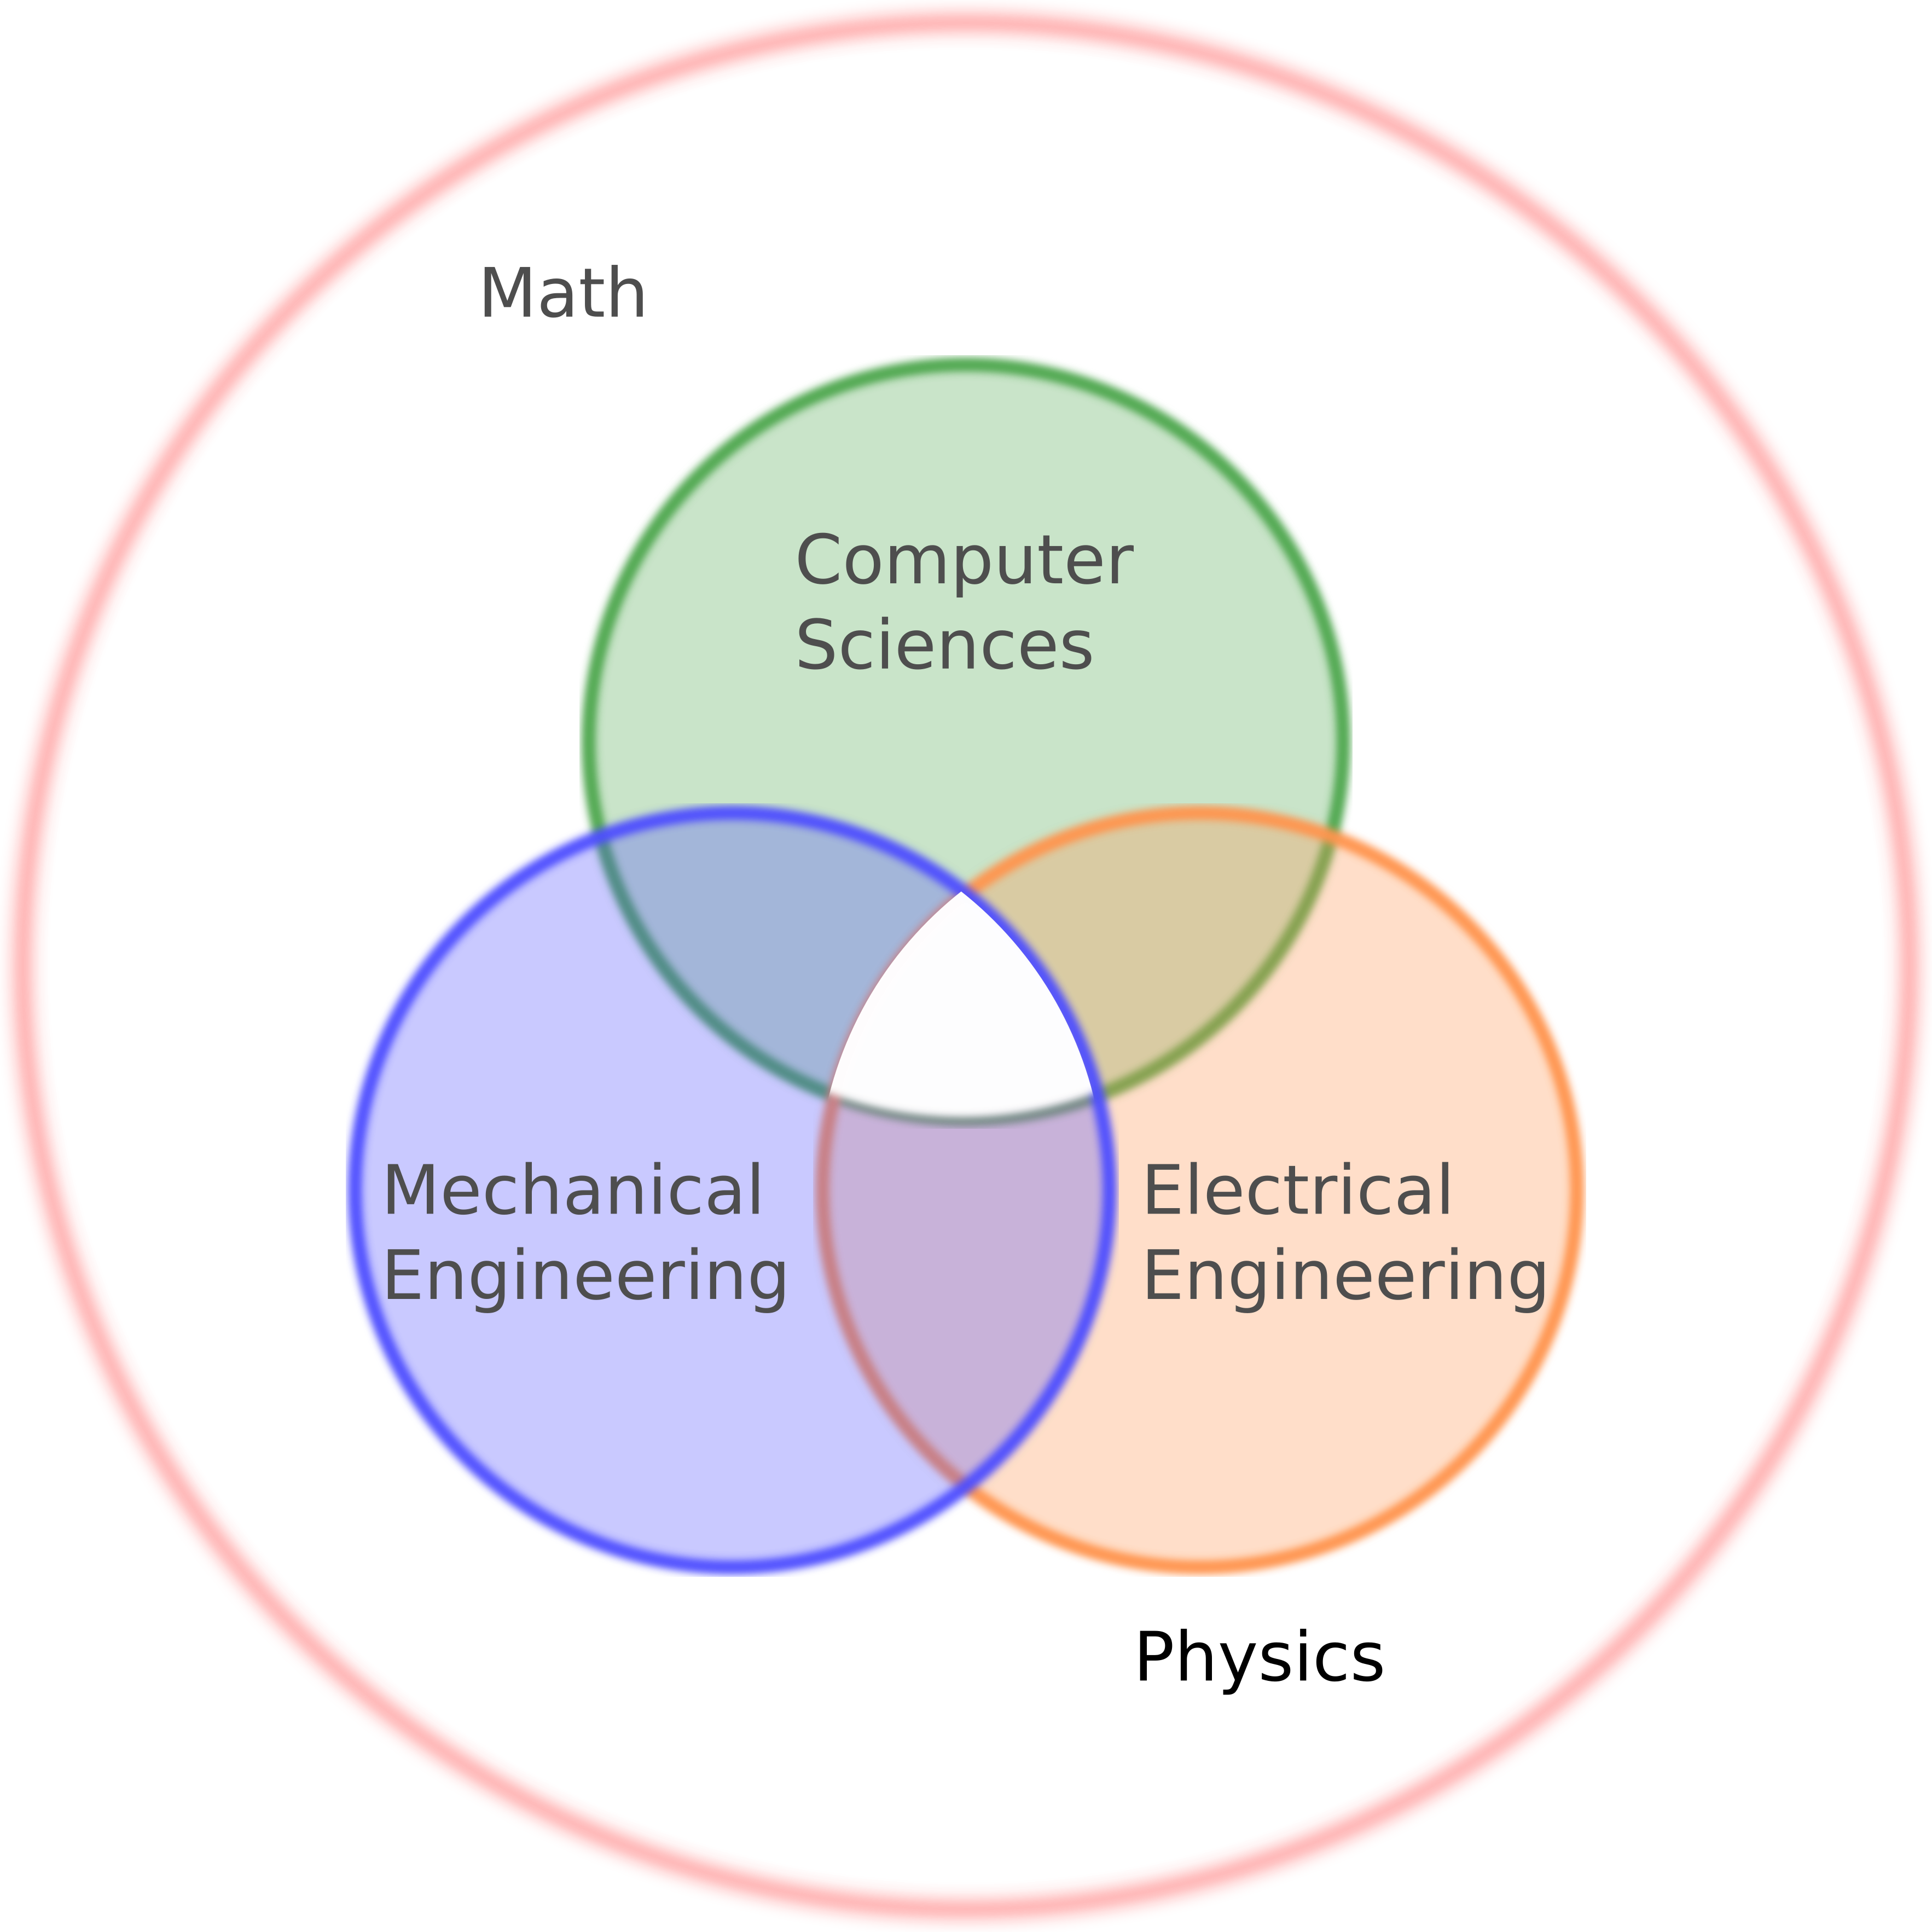
\includegraphics[width = 0.5\textwidth]{./pics/robotics_motivation.png}
    \end{figure}

  }

  \frame{
    \frametitle{Modeling Approaches}
    \begin{column}{0.5\textwidth}
    Bottom Up
      \begin{itemize}
        \item A model consists of submodels
        \item Every parameter is considered
        \item High physical accuracy
      \end{itemize}
    \end{column}%
    \begin{column}{0.5\textwidth}
    Top Down
    \begin{itemize}
      \item A model consists of an input-output behavior
      \item A subset of parameters are needed
      \item Efficient simulation
    \end{itemize}
    \end{column}%
  }

  \frame{
  \begin{column}{0.5\textwidth}
  Bottom Up
    \begin{itemize}
      \item (Low Level) Controller Design
      \item Learning more than I/O relations
      \item More "realistic" behavior
    \end{itemize}
  \end{column}%
  \begin{column}{0.5\textwidth}
  Top Down
    \begin{itemize}
      \item (High level) controller design
      \item Learning basic I/O relations
      \item Visual behavior / Gaming
    \end{itemize}
  \end{column}
  }


  \frame{
    \frametitle{Motivating Example}

    Task \\
    Model a factory worker which can step in the working cell of a robot.
    The robot is able to identify a worker via visual detection. \newline

    Abstraction \\
    Model a visual of the factory worker that is able to "walk" in the simulation.\newline

    More Abstraction \\
    Model a visual of the factory worker that is able to change its position smoothly.
  }

  \frame{
    \frametitle{Motivating Example II}

    Task \\
    Estimate the forces acting on each joint during a given walking gait. \newline

    Abstraction \\
    High accuracy simulation of a robots lower body. \newline

    Questions \\
    Is a rigid body simulator sufficient for the task?
  }

  \section{Opportunities and Limitations}

  \frame{
    \frametitle{Soft Body Dynamics}
  }

  \frame{
    \frametitle{Good Questions}

    How to model clearance in joints? \newline

    How to make objects grippable? \newline

    How to avoid self collisions?

  }

  \frame{
    \frametitle{"Nonphysical" Models}
    Task \\
    Model a factory worker which walks around naturally. \newline

    Abstraction \\
    Give a model a walking like behavior. \newline

    Needs \\
    Ray Tracing: Detects objects in front of it. \\
    Target Generator: Creates a (reachable) target.

  }


    \frame{
      \frametitle{"Nonphysical" Models}
      Task \\
      Model a factory worker which walks around naturally. \newline

      Abstraction \\
      Give a model a walking like behavior. \newline

      Solutions \\
      Look at gaming AI. Many algorithms are present.\\
      Maybe a simple control strategy is sufficient?
    }


    \frame{
      \frametitle{"Nonphysical" Models}
      Task \\
      Model a current for underwater simulations. \newline

      Solution \\
      Create a vectorfield of current forces and add some degree of randomness! \newline

      Hint \\
      Same goes for for aerial forces.
    }
  \section{Coupling of Domains}

  \frame{
    \frametitle{Interdisciplinary Modeling}

    IMAGE OF MODEL CHAIN HERE
  }

  \frame{
    \frametitle{Model of an IMU}
  }

  \frame{
    \frametitle{Connect a DC Motor}

  }

  \section{Simulationtools}

  \frame{
    \frametitle{MARS}
  }


  \frame{
    \frametitle{Gazebo}
  }

  \frame{
    \frametitle{Simulink}
  }

  \frame{
    \frametitle{OpenModelica}
  }


\end{document}
